\documentclass{article}
\usepackage[utf8]{inputenc}
\usepackage{amsmath}
\usepackage{amssymb}
\usepackage{changepage}
\usepackage{graphicx}
\title{Homework 3a Writeup}
\author{Michael Tang}
\date{due May 14, 2019}
\begin{document}
\maketitle
\begin{adjustwidth}{-2cm}{-2cm}
\section{Usage}
Use ``make a'' to compile and link the modules from utils and from the root directory. DO NOT use ``make'' - this will be used to link all the required files for Part b. ``make clean'' is available to remove all .o files.\\
Execute the program as follows:\\
./locks [-n \textit{nthreads}] [-L \textit{lockmode}] [-f \textit{fair}] [-o \textit{outpath}]
\begin{itemize}
	\item -n specifies number of threads, and will run the program in parallel mode if $n \geq 1$. To run in serial mode, use -n 0. n also must divide $BIG$ cleanly, where as of this time of writing $BIG = 2725408$.
	\item -L specifies lock type, 0-3 for TASLock, PThread\_Mutex, ALock, and CLHLock in sequence. -L specification is required if $n > 0$.
	\item -f is a fairness flag, 0 for no enforced fairness and 1 for fairness. When $f = 1$ (which is the default value unless specified otherwise), each thread will be restricted to count to $BIG/n$. When $f=0$, the program will stop when the counter has reached $BIG$ and each thread can do any amount of work.
	\item -o is the path for the file to which user wants to output. If not specified, program will default to stdout. \textbf{WARNING:} files open in append mode. If you want to start a clean version of existing output files make sure to remove them first.
\end{itemize} 

\section{Design Changes}
In the input/initialization phase, after learning in class that we were to normally restrict each thread to doing $BIG/nthreads$ increments, I added the -f argument at the command line to enable me to remove that restriction and run my fairness experiment.\\
For lock design:
\begin{itemize}
	\item CLHLock design was changed to improve performance by only mallocing as many nodes as there are threads during lock initialization, instead of mallocing and freeing nodes as we go. To ensure that a node attempting to grab the lock again after unlocking did not, in the process, prevent the next node from exiting the lock, the address for a thread's node was "shuffled" every unlock by being set to the address of its predecessor node. This actually required $nthreads + 1$ nodes with an initial tail node allocated to allow threads to shuffle spaces without colliding, but allowed for much better performance.
	\item CLHLock and ALock were adjusted to use the PaddedPrimBool\_t structure provided by paddedprim.h to prevent false sharing in the cache, and further improve performance.
	\item Creation and destroy() calls were added for each type of lock for modularity's sake, specifically for easier use in Part b. 
	\item TryLock now specifically returns 0 on successful lock grab and -1 on busy lock.
\end{itemize}
My initial thought that $BIG$ would only have to be reduced from 2323 was incorrect. For correctness testing, except for the skewed time test, $BIG$ was set to 681352 for robustness. Only in the skewed time test was $BIG$ reduced to 123 because a 1 second sleep time is introduced in the critical section, rendering larger $BIG$ values too slow in testing.\\
For performance testing, $BIG$ was set to 2725408, because at 681352 the variance of runtimes was too large. At larger numbers, runtime was too long and occasionally variances of thread work were too large to be held by \textit{unsigned long long}. 2725408 was also picked because it is cleanly divided by 1, 2, 4, 8, and 14, the $nthreads$ needed for the experiments.

\section{Testing Results}
\subsection{Correctness}
The invariants to be tested were:
\begin{itemize}
	\item Mutual exclusion
	\item Correct final counter value, and thread portion restriction when required
	\item Ordering, for the FIFO locks
\end{itemize}
All tests are available in the tests folder, and correctness tests have ``correctness'' in their name, except for ``skewedtest.txt''.
\subsubsection{Mutual Exclusion}
To test mutual exclusion, a shared array of length $BIG$ was passed to every thread where each slot $i$ represents the number of times the counter value $i+1$ was encountered, initialized to 0. Threads incremented at a slot $i$ if the counter was at that value $i+1$ when they accessed it. If mutual exclusion was violated and two or more threads were allowed to enter the critical section at the same time, slot $i+1$ would have value 2 or more. After all threads conclude operations and right before the program exits, this array is checked for any values greater than 1; if there are any, then they would be outputted in the format: ``Mutex failure at counter: $i+1$. Number of threads that reached CS: $n$'', where $n$ is the number of threads that reached CS at the same time.\\
For good measure, a skewed time test was also used where ``sleep(1)'' was called in the CS, to ensure fully robust mutual exclusion.\\
TASLock and PThreads were tested with $nthreads = 1, 2, 4, 8, 14, 56, 1288$ for normal tests, and CLHLock and ALock with $nthreads = 1, 2, 4, 8, 14, 56$, because 1288 could not run fast enough. For the skewed time test all locks were tested with $nthreads = 56$.\\
In none of the tests was the failure message printed, so we can safely conclude that all lock implementations uphold mutual exclusion.
\subsubsection{Counter Value and Division}
Each thread also received a slot in an array of individual counts with an int initialized to 0. Slot $t$ was incremented every time thread $t$ incremented the counter. In the correctness tests besides skewedtest final individual thread increment counts were printed, and in every test the final counter value was printed.\\
All of the tests had the correct amount ($BIG/nthread$) of incrementations for each thread, and the correct final counter value.
\subsubsection{FIFO Lock Ordering}
FIFO ordering was not explicitly tested because it was decided to be too slow or complicated. Instead, FIFO ordering was implicitly tested by observing mutual exclusion, final counter value, correct thread division when fairness was enforced, and fairness when it was not enforced (-f 0). The first three measures were already observed to be accomplished above. As observed in the third performance experiment below, fairness was also higher for the FIFO locks than for pthread\_mutex or TASLock at higher thread counts. Therefore, we can reasonably conclude that the FIFO ordering of CLHLock and ALock are respected in this implementation.

\subsection{Performance}
All performance test outputs are available in hw3/tests, and data was put through Jupyter notebooks using Python 3 and the Pandas package to output the needed data tables. The notebooks can also be found in tests and are labelled according to their experiment. For the first two tests, individual thread count and variance measurement were commented out to reduce their effects on runtime measurements, especially due to the memory calls they involve.
\subsubsection{Idle Lock Overhead}
Tests were run as specified with $nthreads = 1$ and the different lock modes taken, as well as serial mode. To reduce variance each lock mode and serial mode was tested 10 times and the runtime averaged across those 10 times for each. Then $BIG$ was divided by that average runtime to get average throughput, and this throughput for each lock divided by the average throughput of serial mode to get the required speedup ratios. The resulting data and graph are below.\\
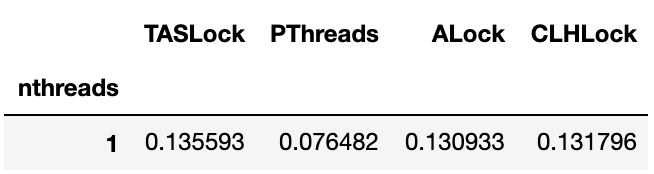
\includegraphics[width=\linewidth]{overheadData.png}\\
\null\\
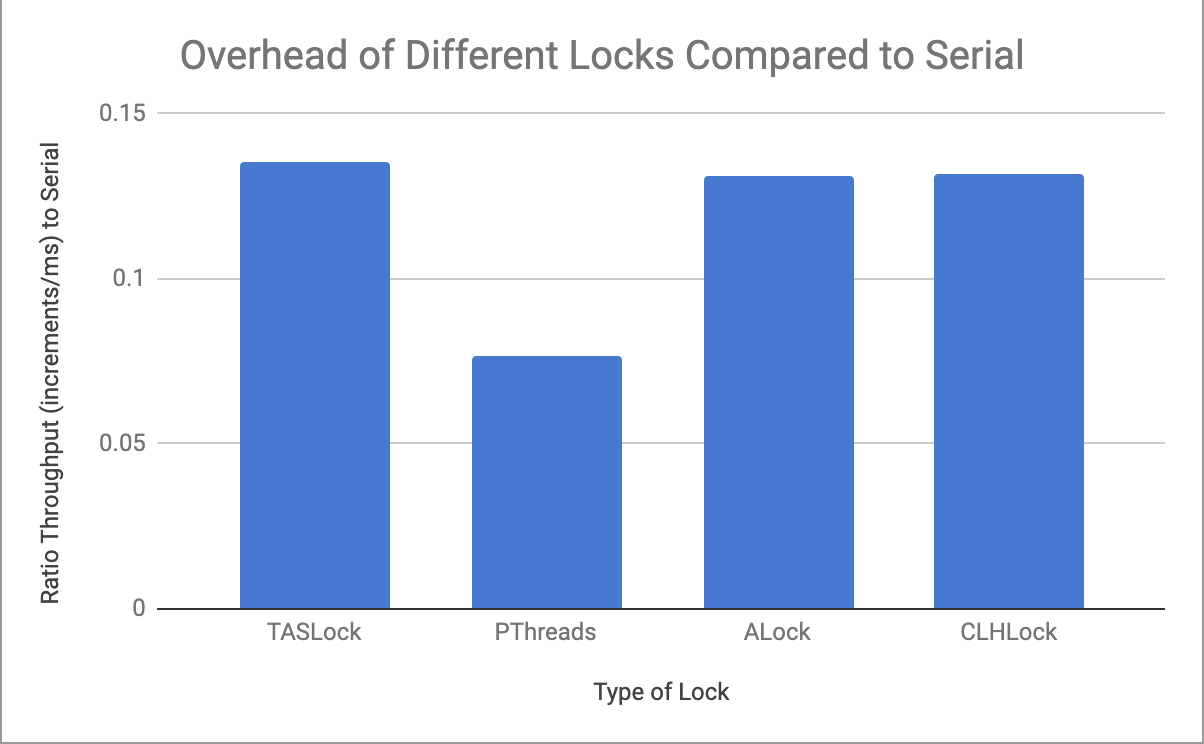
\includegraphics[width=\linewidth]{overheadGraph.png}\\
As hypothesized, TASLock and ALock had similar overhead. CLHLock also had a similar overhead to those two because of the new implementation mallocing a set number of nodes at the beginning of the program. As hypothesized in class, all three lock implementations had lower overhead (higher speedup) than pthread\_mutex, likely due to the use of system calls in pthread\_mutex.
\subsubsection{Lock Scaling}
Tests were run as specified again with $nthreads = \{1, 2, 4, 8, 14\}$ and the different lock modes. Again 10 trials were taken for each lock mode and serial mode, and the runtime averaged out then the throughput and throughput ratios calculated. The resulting data and graph are below.\\
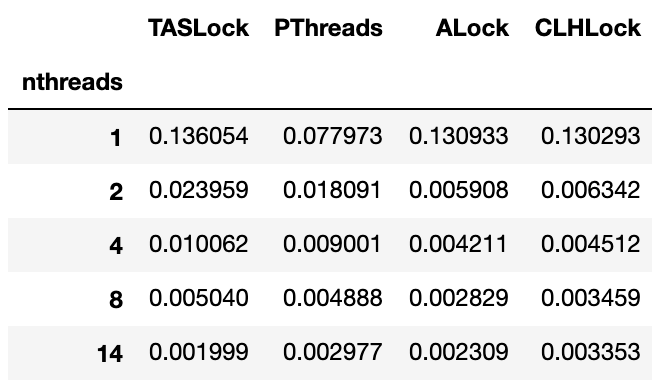
\includegraphics[width=\linewidth]{scalingdata.png}\\
\null\\
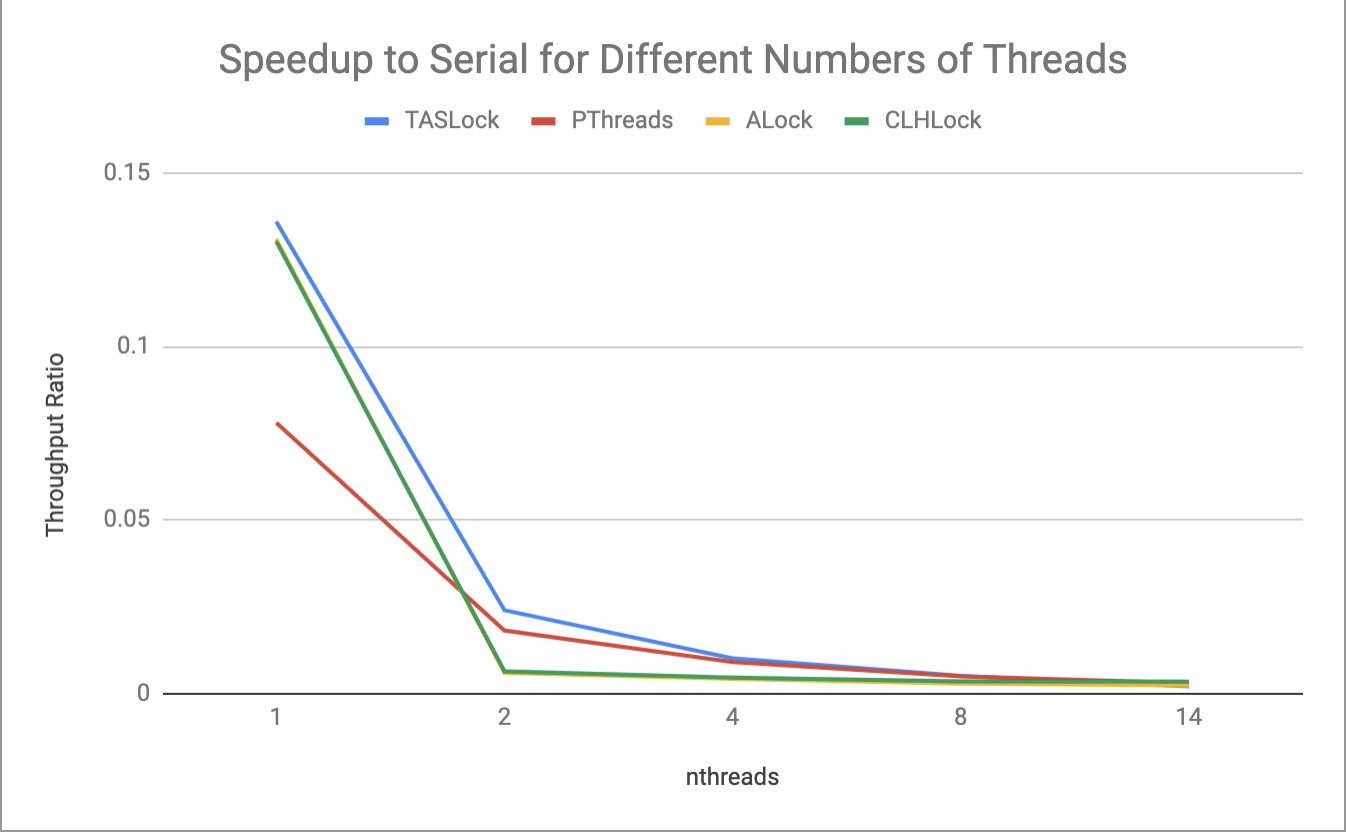
\includegraphics[width=\linewidth]{scalinggraph.png}\\
Contrary to the hypothesis, TASLock did not experience a faster decrease in speedup compared to ALock or CLHLock, the two of which had very similar speedup data due to the design change to CLHLock. Both experienced higher decline in speedup than pthread\_mutex. This could be explained by the additional address operations required at $nthreads > 1$ adding significant runtime burden to ALock and CLHLock.\\
At $nthreads=14$ TASLock was the slowest lock as hypothesized and also experienced the biggest proportional drop in speedup from $nthreads=8$\; speedup ratio at $nthreads=8$ was 2.5x that of $nthreads=14$. A possible explanation for this trend is that while at lower $nthreads$ the system calls of pthread\_mutex and the memory handling overhead of ALock and CLHLock accounted for a significant amount of the overhead, starting from $nthreads=14$ onwards we were likely to see the contention overhead become more significant. At this point, as the data shows, the other three locks become faster.\\
I also venture to explain this as the cause for ALock and CLHLock being slower than pthread\_mutex for $nthreads = \{2,4,8\}$. At $nthreads=14$ ALock and pthread\_mutex were close, and CLHLock was faster. This leads me to believe that beyond $nthreads=14$ the contention overhead being more significant would also render pthread\_mutex slower than ALock and CLHLock.\\
\subsubsection{Personal Test: Lock Fairness}
To test fairness, I set flag -f to 0 at command line to remove requirements on how many increments each thread should do, letting each thread do as much work as they could. Then I took the variance of individual thread increments from the mean amount of increments, which would be $BIG/nthreads$. This test was performed for $nthreads = \{1,2,4,8,14\}$  and all lock types. 10 trials were also conducted for each lock mode and the variance averaged out over those 10 trials. The resulting data and graph are below.\\
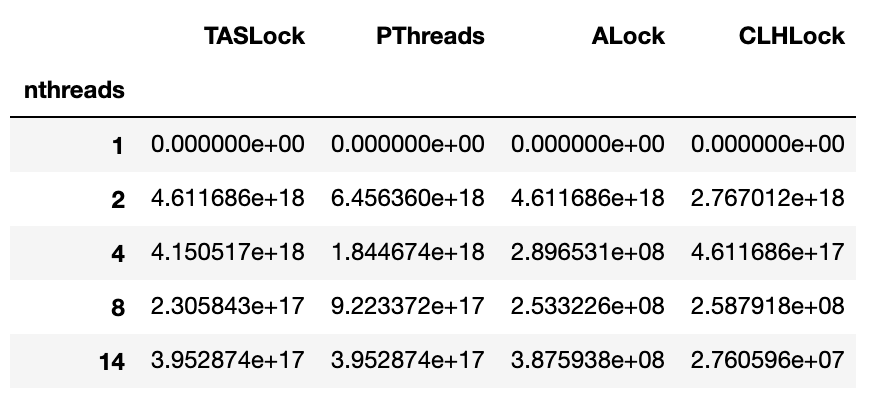
\includegraphics[width=\linewidth]{fairdata.png}\\
\null\\
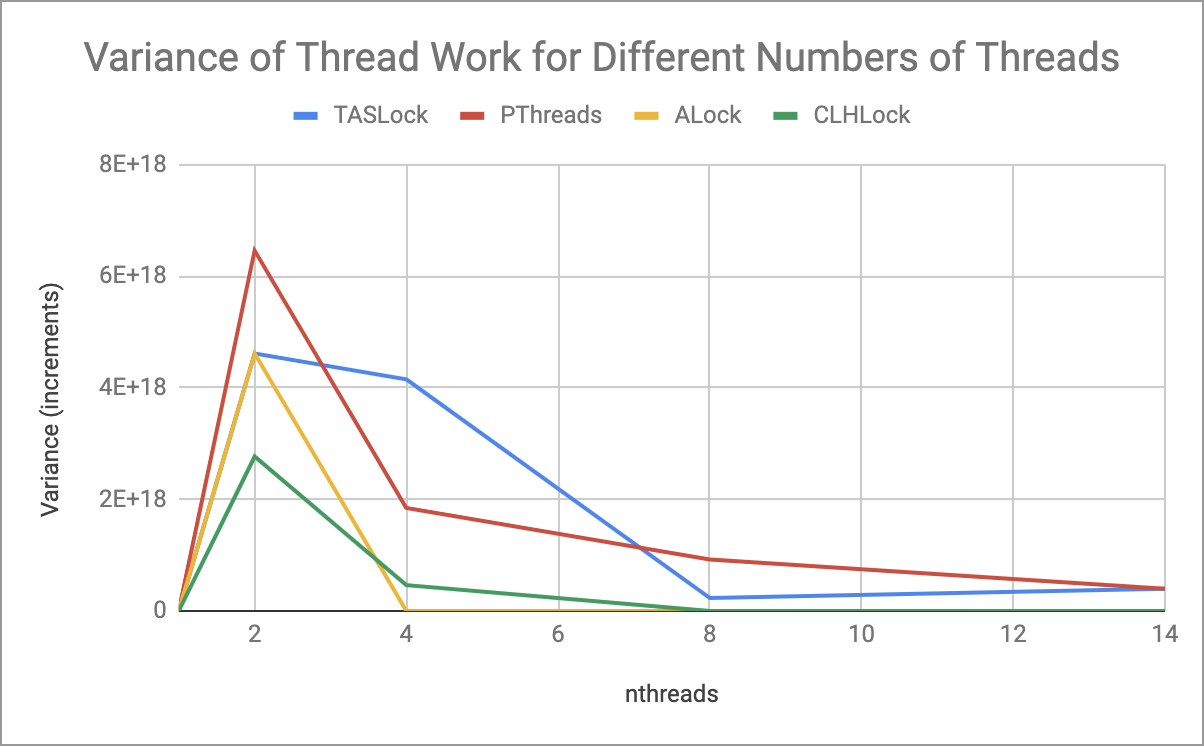
\includegraphics[width=\linewidth]{fairgraph.png}\\
What went against the hypothesis was that variance of thread work for all locks tended to \textit{decrease} as $nthreads$ increased. This is disregarding $nthreads=1$ because at that point the variance is clearly equal to 0, as the solitary thread must do $BIG = BIG/1 = BIG/nthreads$ work. A possible explanation for this is that at $nthreads=2$, the second thread that is unable to obtain the lock could be spinning at tryLock() instead of the lock itself. The memory reference of tryLock is slower than in the lock itself, and would enable the first thread to unlock and re-grab the lock before the second thread can grab it. This effect is reduced at higher amounts of $nthreads$ as threads are able to enter the section where they spin on the lock, and are less easily starved out by the faster threads.\\
At $nthreads=2$ CLHLock experiences nearly half the variance of the other locks. This could be accounted for by the node address change required of a thread calling unlock(), which is slower than the unlock() processes of the other locks and would less often outpace the attempts of the second thread to grab the lock.\\
In agreement with the hypothesis, the variance of thread work for TASLock and pthread\_mutex remained higher than that of CLHLock and ALock at $nthread > 2$. This suggests that the fairness theoretically enforced by the FIFO-queue nature of the latter two locks is present. Due to their similar queue nature and the more efficient design of CLHLock the latter two locks are also very similar in variance at higher $nthread$, as hypothesized.\\
For future tests, removing $nthreads=1$ and adding another level greater than 1 would be better. 
\end{adjustwidth}
\end{document}
